\documentclass[aspectratio=169]{ctexbeamer}
\usepackage[T1]{fontenc}
\usepackage{latexsym,amsmath,xcolor,multicol,booktabs,calligra}
\usepackage{graphicx,listings,stackengine}
\usepackage{hyperref}

\usepackage{PekingU}

% 去掉每节/子节前面的自动目录页
\AtBeginSection[]{}
\AtBeginSubsection[]{}

% ===== 每节课改这里 =====
\author{Cap1taL}
\title{各类动态规划}
\subtitle{6:20开始按车号上车，6:50早餐是随车配发，餐食统一在大巴车上分发！转自组委会:我们会与校医核实，如果存在教练故意编造理由请假，将影响明年学校其他名额审批。
明天社会实践活动请所有同学参加，我们是一个集体，代表？？，今天只有？？的学生在请假，校医反映都是水土不服，可是精神状态都不错。如果这些学校学生继续不服从组委会安排，后面计算机学会将对这些学校申请参赛的名额进行限制！同时也会影响??的参加名额。请各位教练三思。}
\date{2026年7月}
% ========================

% 代码高亮设置
\definecolor{deepblue}{rgb}{0,0,0.5}
\definecolor{deepred}{rgb}{0.6,0,0}
\definecolor{deepgreen}{rgb}{0,0.5,0}
\definecolor{halfgray}{gray}{0.55}

\lstset{
    basicstyle=\ttfamily\small,
    keywordstyle=\bfseries\color{deepblue},
    emphstyle=\ttfamily\color{deepred},
    stringstyle=\color{deepgreen},
    numbers=left,
    numberstyle=\small\color{halfgray},
    rulesepcolor=\color{red!20!green!20!blue!20},
    frame=shadowbox,
}

\begin{document}

\kaishu

% 封面
\begin{frame}
    \titlepage
\end{frame}

% 目录
% \begin{frame}{目录}
%     \tableofcontents[sectionstyle=show,subsectionstyle=show/shaded/hide,subsubsectionstyle=show/shaded/hide]
% \end{frame}

% ===== 从这里开始写你的内容 =====

\section{前言}

\begin{frame}{动态规划……？}
    大家觉得什么是动态规划？动态规划在解决什么问题？什么问题需要动态规划？

    为什么会有各种各样的“动态规划种类”？
    
    他们之间到底有什么区别？又有什么共性？
\end{frame}

\begin{frame}{规划}
    这一部分的前两节课我们预计处理六种 DP（不含树上）
    
    有部分种类会着重练习

    每次课我们处理三种 DP 类型

    然后我们会有一次状态设计的强化

    最后是DP优化
\end{frame}

\section{背包DP}

\begin{frame}{常见的模板背包}
    \begin{itemize}
        \item 0-1 背包DP
        \begin{itemize}
            \item 滚动数组
        \end{itemize}
        \item 完全背包
        \item 多重背包
        \begin{itemize}
            \item 二进制分组
        \end{itemize}
        \item 多费用背包
        \item 分组背包
        \item 依赖背包
    \end{itemize}
\end{frame}

\subsection{Codeforces 1428G2 Lucky Numbers (Hard Version)}
\begin{frame}{Codeforces 1428G2 Lucky Numbers (Hard Version)}
    幸运数字为 $3,6,9$。一个数的十进制表示中，每位有一个幸运值 $F_j$，若该位数字 $d$ 是 $3,6,9$ 之一则贡献 $\frac{d}{3}\cdot F_j$，否则贡献 $0$。
    
    第 $i$ 只羊要写出恰好 $k$ 个非负整数，和为 $n_i$，最大化幸运值之和。

    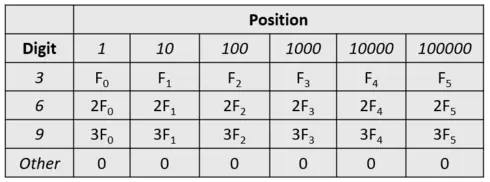
\includegraphics[scale=0.5]{pic/1.png}
    
    $k\le 999999,\ q\le 10^5,\ n_i\le 999999$
\end{frame}

\subsection{洛谷 P16714 玲珑}
\begin{frame}{洛谷 P16714 玲珑}
    $N$ 根小木棍，长度 $a_i$，染成红绿蓝三色之一。将所有同色木棍首尾相接拼成长木棍，判断三条长木棍能否拼成三角形。
    
    求满足条件的染色方案数，对 $998244353$ 取模。
    
    $N\le 200,\ a_i\le 500$
\end{frame}

\subsection{Codeforces 601E A Museum Robbery}
\begin{frame}{Codeforces 601E A Museum Robbery}
    展品有价值 $v_i$ 和质量 $w_i$。支持添加、删除展品，并询问容量为 $1..k$ 的背包最大价值之和的哈希值：
    $$\sum_{m=1}^k s(m)\times p^{\,m-1}\bmod (10^9+7)$$
    其中 $s(m)$ 为容量 $m$ 时的最大价值。
    
    最多 $10^4$ 次添加，$q\le 3\times10^4$，$k,w\le 10^3$
\end{frame}

\subsection{AtCoder agc049\_d Convex Sequence}
\begin{frame}{AtCoder agc049\_d Convex Sequence}
    长度为 $N$ 的非负整数序列 $A$，满足：
    \begin{itemize}
        \item $\displaystyle\sum_{i=1}^N A_i = M$
        \item 对任意 $2\le i\le N-1$，$2A_i \le A_{i-1}+A_{i+1}$（凸性）
    \end{itemize}
    求序列个数，对 $10^9+7$ 取模。
    
    $N,M\le 10^5$
\end{frame}


















\section{区间DP}

\begin{frame}{常见的区间DP}
    \begin{itemize}
        \item 区间DP
        \item ？
    \end{itemize}
\end{frame}

\subsection{洛谷 P9746 合并序列}
\begin{frame}{洛谷 P9746 合并序列}
    给定序列 $a$。每次操作选择 $i<j<k$ 满足 $a_i\oplus a_j\oplus a_k=0$，将 $a_i..a_k$ 替换为它们的异或和。判断能否使序列长度为 $1$，并输出方案。
    
    多组数据，$n\le 500,\ a_i<512$
\end{frame}

\subsection{洛谷 P4170 涂色}
\begin{frame}{洛谷 P4170 涂色}
    初始无色的长度为 $n$ 的木板，每次可将一段连续区间涂成任意颜色，后涂覆盖先涂。求达到目标颜色串的最少涂色次数。
    
    $n\le 50$
\end{frame}

\subsection{Codeforces 1987F2 Interesting Problem (Hard Version)}
\begin{frame}{Codeforces 1987F2 Interesting Problem (Hard Version)}
    给定数组 $a$。每次操作选择一个 $i$ 满足 $a_i=i$，删除 $a_i$ 和 $a_{i+1}$，剩余部分拼接。求最多操作次数。
    
    多组数据，$\sum n\le 800$
\end{frame}

\subsection{AtCoder abc261\_g Replace}
\begin{frame}{AtCoder abc261\_g Replace}
    给定字符串 $S,T$ 和 $K$ 种操作：将单个字符 $C_i$ 替换为字符串 $A_i$，代价 $1$。求将 $S$ 变为 $T$ 的最小总代价，或输出 $-1$。
    
    $|S|\le|T|\le 50,\ K\le 50$
\end{frame}

\subsection{Codeforces 2018F3 Speedbreaker Counting (Hard Version)}
\begin{frame}{Codeforces 2018F3 Speedbreaker Counting (Hard Version)}
    $n$ 个城市排成一行。第 $1$ 时刻征服起始城市，之后每时刻可征服一个与已征服城市相邻的城市。若城市 $i$ 在 $\le a_i$ 时刻被征服则获胜。
    
    对每个 $0\le k\le n$，统计有多少个数组 $a[1..n]$（$1\le a_i\le n$）使得恰有 $k$ 个起始城市可获胜。答案对给定质数 $p$ 取模。
    
    多组数据，$\sum n\le 3000$
\end{frame}












\section{状压DP}

\begin{frame}{常见的状压DP}
    \begin{itemize}
        \item ？！状压 DP？！
        \item 枚举子集的复杂度证明？
    \end{itemize}
\end{frame}

\subsection{Codeforces 1316E Team Building}
\begin{frame}{Codeforces 1316E Team Building}
    从 $n$ 人中选 $p$ 人安排到 $p$ 个不同位置，再从剩下的人中选 $k$ 人作为观众。第 $i$ 人做观众贡献 $a_i$，在位置 $j$ 贡献 $s_{i,j}$。求最大总力量值。
    
    $n\le 10^5,\ p\le 7$
\end{frame}

\subsection{Codeforces 111C Petya and Spiders}
\begin{frame}{Codeforces 111C Petya and Spiders}
    $n\times m$ 棋盘，每格一只蜘蛛。每只蜘蛛可向上/下/左/右走一格或停在原地，不能出界。求最多能空出的格子数。
    
    $n\cdot m\le 40$
\end{frame}

\subsection{洛谷 P7718 Equalization}
\begin{frame}{洛谷 P7718 Equalization}
    给定序列 $a[1..n]$。每次操作选 $l,r,x$，将 $a_l..a_r$ 均加上 $x$。求使所有元素相等的最少操作次数及方案数。
    
    $n\le 18$
\end{frame}

\subsection{AtCoder arc222\_d Shift and Add}
\begin{frame}{AtCoder arc222\_d Shift and Add}
    给定正整数序列 $A,B$，构造 $X$：$X_0=0$，对 $i=1..N$ 可选择 $X_i=10X_{i-1}+A_i$ 或 $10X_{i-1}+B_i$。
    
    对每个 $k$，求 $X_k$ 所能取得的最小数位和（十进制各位数字之和）。每个 $k$ 独立计算。
    
    $N\le 2\times10^4$
\end{frame}


% ===== 结束页 =====

\begin{frame}
    \begin{center}
        {\Huge\calligra Thanks!}
    \end{center}
\end{frame}

\end{document}
